\documentclass[11pt]{article}
\usepackage{geometry}
\usepackage{amsmath,amssymb,amsthm,trace, physics, xfrac}
\usepackage{gensymb}
\usepackage[table,xcdraw]{xcolor}
\usepackage{titlesec}
\usepackage{fontspec}
\usepackage{graphicx}
\usepackage[titletoc]{appendix}
\usepackage{listings}
\usepackage{xcolor}
\usepackage{lipsum}
\usepackage{polyglossia}
\usepackage{tikz}
\usepackage{fancyhdr}
\usepackage[backend=biber,style=numeric, sorting=none, refsegment=section]{biblatex}
\usepackage{multicol}
\usepackage{subfiles}
\usepackage{hyperref}
\usepackage{coffee4}


\setmainfont{GFS Didot}

\setmainlanguage{english}

\urlstyle{rm}
\addbibresource{Files/biblio.bib}

\definecolor{blue}{cmyk}{0.8, 0.5, 0, 0}
\definecolor{codegreen}{RGB}{0,204,0}
\definecolor{codegray}{RGB}{225,225,225}
\definecolor{codepurple}{RGB}{255,80,255}
\definecolor{codered}{RGB}{255,80,80}

\newcommand{\hsp}{\hspace{5pt}}
\titleformat{\section}[hang]{\Large\bfseries}{\thesection\hsp\textcolor{blue}{$\mid$}\hsp}{0pt}{\Large\bfseries}
\titlespacing{\section}{10pt}{0pt}{15pt}

\titleformat{\subsection}[hang]{\large\bfseries}{\thesubsection}{5pt}{\large\bfseries\underline}
\titlespacing{\subsection}{15pt}{15pt}{5pt}


\geometry{a4paper,top=2.2cm,bottom=3cm,left=2.5cm,right=2.5cm,heightrounded}

\pagestyle{fancy}
\fancyhf{}
\rhead{}
\lhead{\leftmark}
\cfoot{\thepage}

\title{\huge{\textbf{\underline{Prehistoric Human Dispersion}}}\\ \Large{The Exodus from Africa}}
\author{Anon}
\date{}
\begin{document}

\maketitle

\cofeAm{0.2}{1}{100}{5cm}{3cm}

\begin{multicols}{2}
\tableofcontents

\section{Timeline of Migration}
The general accepted theory is that the first humans emerged in the Horn of Africa (Modern Day Ethiopia, Somalia and Eritrea), about 190-200 thousand years ago\cite{EOBO, BEBO} and later moved out of Africa (OoA hypothesis) in either a single or in multiple dispersal waves.
\subsection{Single Dispersal Model}
In the case of a single dispersal model, the question becomes which of the available routes were used, with the common consensus being that either a north path through Egypt and the Levant was followed or a south route via the coastline of Arabia and Iran (Fig. 1).\\
\textbf{North Path} The evidence for the North Path are scarce and mostly indicate to a failed exodus at around 90 thousand years ago \cite{EOBO}, although there are still genetic studies that indicate to the possibility of a Northern path, based on the study of Y chromosome haplogroups\cite{LEVA} and the sequencing of genomes of people currently living in the hypothetical Northern Route\cite{EGPT}.\\
\textbf{South Path} The Southern Route is supported by mitochondrial DNA, as well as by Short Tandem Repeats models, alongside an analysis of LD decay\footnote{The chromosomal or genomic location of a gene or any other genetic element is called a locus (plural: loci) and alternative DNA sequences at a locus are called alleles. Linkage disequilibrium (LD) is the non-random association between alleles at different loci in a breeding population.}, although the archaeological evidence has been extremely limited.


\subsection{Multiple Dispersal Model}
The first multiple dispersal model was proposed around 1994 by Lahr and Foley \cite{AAA}, suggesting a first migration wave through the southern route, at around 50-100 thousand years ago, and another following the northern route around 40-50 thousand years ago. McEvoy et al \cite{MCEV} also suggested a more complex migration that a single wave dispersal, by studing divergence times in Eurasian populations and also including intermixing between anatomically modern humans (AMH) and Denisovans and Neanderthals\footnote{Unfortunately the contraints of this report do not allow us to go in depth, but Denisovans and Neanderthals are extinct human species (or subspecies) that populated Eurasia before "we" (Homo Sapiens) reached those areas.}.\\
Recent work has also suggested heavily that accounting for intermixing between AMH and Neanderthals and Denisovans, the multiple dispersal model seems more likely\cite{TEMP}.
\end{multicols}

\begin{figure}[h!]
    \centering
    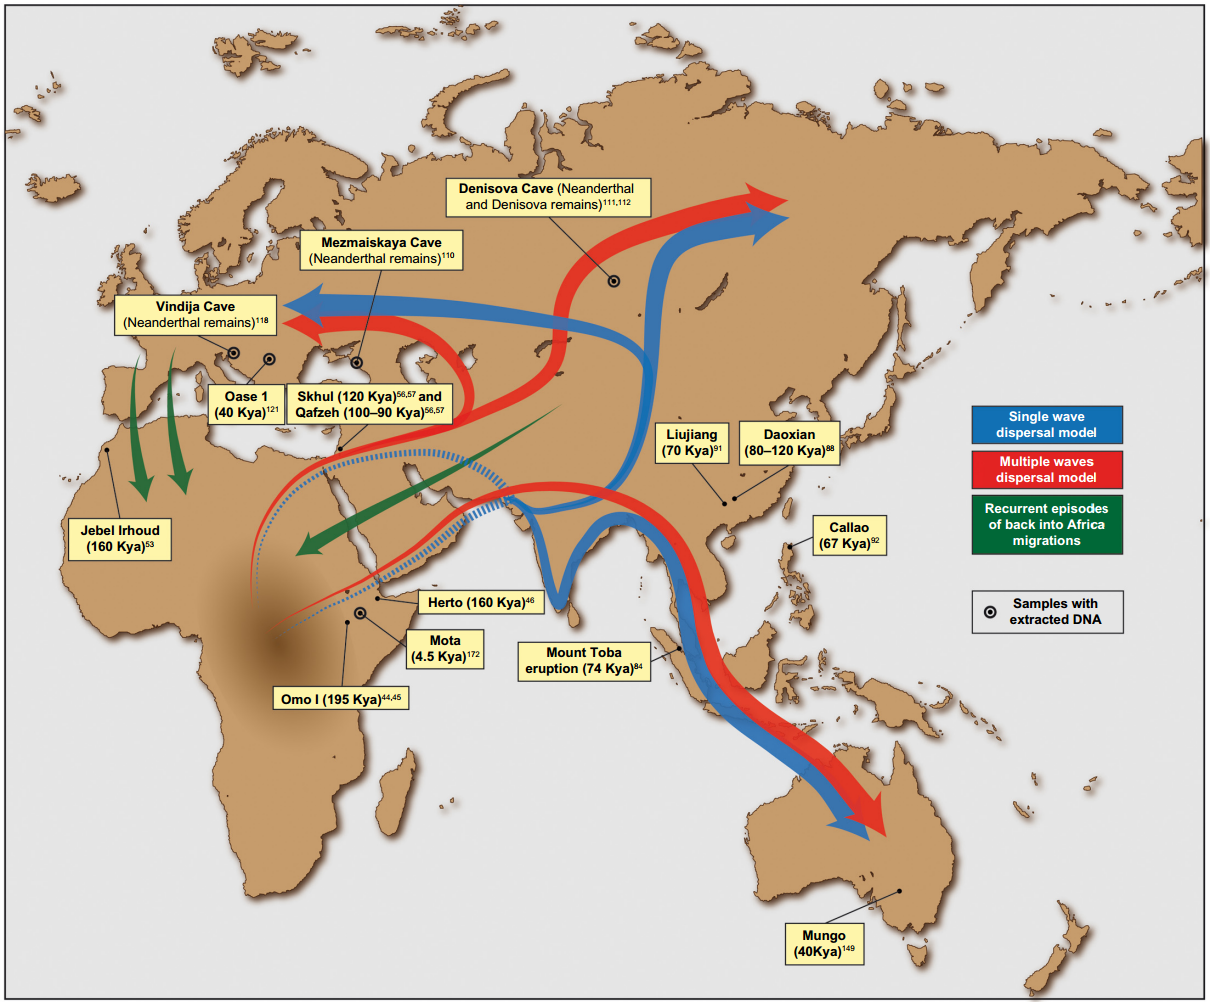
\includegraphics[scale=0.4]{Files/Images/migrationwaves.png}
    \caption{Different models of human spread around Afroeurasia. Red arrows indicate the Multiple Dispersal Model, Blue arrows the Single Disperal Model and Green Arrows indicate possible migrations back to Africa.}
\end{figure}


\begin{multicols}{2}

\section{Introduction to Q-Learning}

Q-Learning is a model-free reinforcement learning algorithm, meaning that it does not depend on a transition probability distribution or a reward function in order to reach the desired result. Rather, the transition probability distribution and the reward function are collectively called the model, and the process of learning is explicitly \textbf{trial and error}. The algorithm has no prior knowledge of the data set and has to explore it, and find special areas in the data set with a high reward, with the ultimate goal of maximising it's rewards.

\subsection{The Technical Details}

Q-learning is an algorithm that is able to find an optimal policy for any Finite Markov Decision Process (FMDP) by maximizing the expected total reward over a collection of successful steps. Given infinite time, the algorithm is able to always identify the optimal policy.\\
As a reinforcement learning algorithm, Q-learning requires an agent, a set of states ($S$), and a set of actions ($A$). For any action $a\in A$, the agents able to change it's state to a new one, and the change rewards the agent with a number. Big positive numbers represent a high reward, low positive numbers a small reward, and a negative value represents a negative reward, so that the agent tries to get away from it. The overall goal of the agent is then to find a policy (path) the maximizes the total reward.\\
Since the agent has no prior knowledge of the environment, it relies upon a set of values on which it relies upon to help it find the optimal policy, like a map. This is called a Q-table.

\subsubsection{Q-Table}

The Q-table is represented as a table of $N+1$ dimensions, with $N$ being the dimensions of the environment and the $N+1$ representing the dimensions of the environment plus the dimension of the actions.\\
A specific Q-value inside the Q-table represents the quality\footnote{Hence the name Q-learning(Quality-learning).} of a specific action $a$ given a specific state $s$ and it represents the agent's estimation of the sum of future rewards. An optimal Q-table allows the agent to make the optimal actions, meaning that the Q-table represents the current policy for acting in the current environment.\\
Since on every action the state changes, we need to find a way to calculate the change of the Q-value for the acting taken, based on the Q-value of the resulting state, which is determined by the reward of the current state, and the expectation of future rewards.

\subsubsection{Temporal Difference}
To achieve this, we use something called Temporal Difference (TD) which is the reward received for the action taken in the previous state, plus the maximum Q-value in the current state, weighted with a discount factor, minus the Q-value of the action of the previous state
\begin{equation*}
    TD(s_{t}, a_{t}) = r_{t}+\gamma\cdot\max_{a}Q(s_{t+1},a)-Q(s_{t},a_{t})
\end{equation*}

where $s_{t}$ is the previous state, $r_{t}$ is the reward in the previous state, $\gamma$ is called the \textit{discount factor}, and $s_{t+1}$ is the current state. The discount factor $\gamma\in(0,1)$ determines the importance of future rewards, with $\gamma$ near zero meaning a greedy\footnote{In the sense of trying to maximise short-term rewards} algorithm, and $\gamma$ close to 1 meaning a long-term reward goal.

\subsubsection{The Bellman Equation}

The Bellman\footnote{Richard Ernest Bellman (1920–1984)} equation is the rule used to update the value for the action taken at the previous state.
\begin{equation*}
    Q_{new}(s_{t},a_{t})=Q_{old}(s_{t},a_{t})+\alpha\cdot TD(s_{t},a_{t})
\end{equation*}

where $\alpha$ is the \textit{learning rate} of the algorithm. The learning rate represents the weight Temporal Difference has on the new value, with a learning rate close to 0 implying that the algorithm is mostly exploiting prior knowledge and not exploring to a significant extent. Meanwhile, a learning rate close to 1 prioritises exploration, and for a deterministic environment it is the ideal value, since this creates ample chances for the agent to explore the entire space.

\section{Simulation of the Migration}

In order to create an algorithm, we chose to use Python, without using the pre-existing libraries (PyTorch, sk-learn), but rather make the algorithm manually, using NumPy.\\
First we  take an image of Afroeurasia and turn it into a bitmap, which is a 2d matrix with 1s and 0s, depending on the color value of the original pixels of the picture and the threshold filter we have set (Fig. 2).\\
For the Q-table we generate a table that is 1920$\times$1254$\times$4, and fill it with Gaussian Noise and for the rewards table we use the bitmap and add some reward locations, and land bridges\footnote{This is because we decentivize the agent from going into the water, to reduce training time.} to match the points of interest at the beginning of the section (Fig. 3). The special reward points are located in Europe, Australia and East Siberia, near the Bering Strait.

\subsection{Applying the algorithm}
The actions that the agent is able to do are: \textbf{go north, go south, go east,} and \textbf{go west}, and at the beginning we can see the agent perform a random walk, based on the Q-table values for each location-action pair (Fig. 4).\\
Once the agent discovers one of the reward. If we let it fully optimise, it discovers the reward locations, but the issue is that because it optimises fully, it draws almost perfect straight lines, which makes the movement of people seem unnatural, since they didn't have previous knowledge of their environment, nor did they have an explicit intent to go to Australia and East Siberia (Fig. 5).\\
This problem is a really difficult problem to solve, since Qlearning is a \textbf{greedy} algorithm, meaning that we cannot spread "breadcrumbs", i.e. low rewards scattered strategically around the map, to help lead the agent to the areas we would want them to go (Fig. 6). This also made incorporating Europe difficult, since the agents would find the European reward point first, and would go exclusively for it, seeing as it is closer to the others.\\
Another problem is that our rewards map is very scarce, i.e. there are big expanses of no rewards present, which greatly increases training time, as in all of those the agent performs longer and wider random walks until it accidentally finds one of the reward points (Fig. 7).
\end{multicols}


\begin{figure}[h!]
    \centering
    \begin{minipage}{0.49\textwidth}
        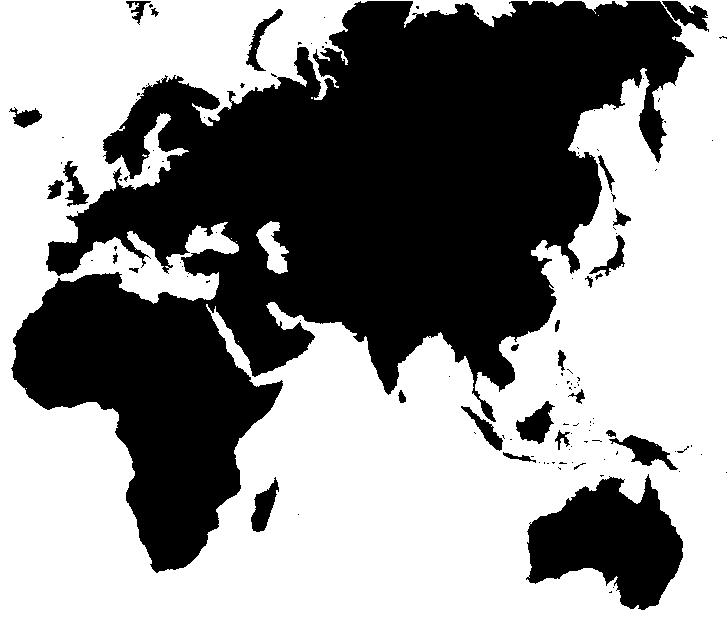
\includegraphics[scale=0.25]{Files/Images/pure-bw-earth.jpg}
        \caption{Bitmap of Afroeurasia.}
    \end{minipage}
    \begin{minipage}{0.49\textwidth}
        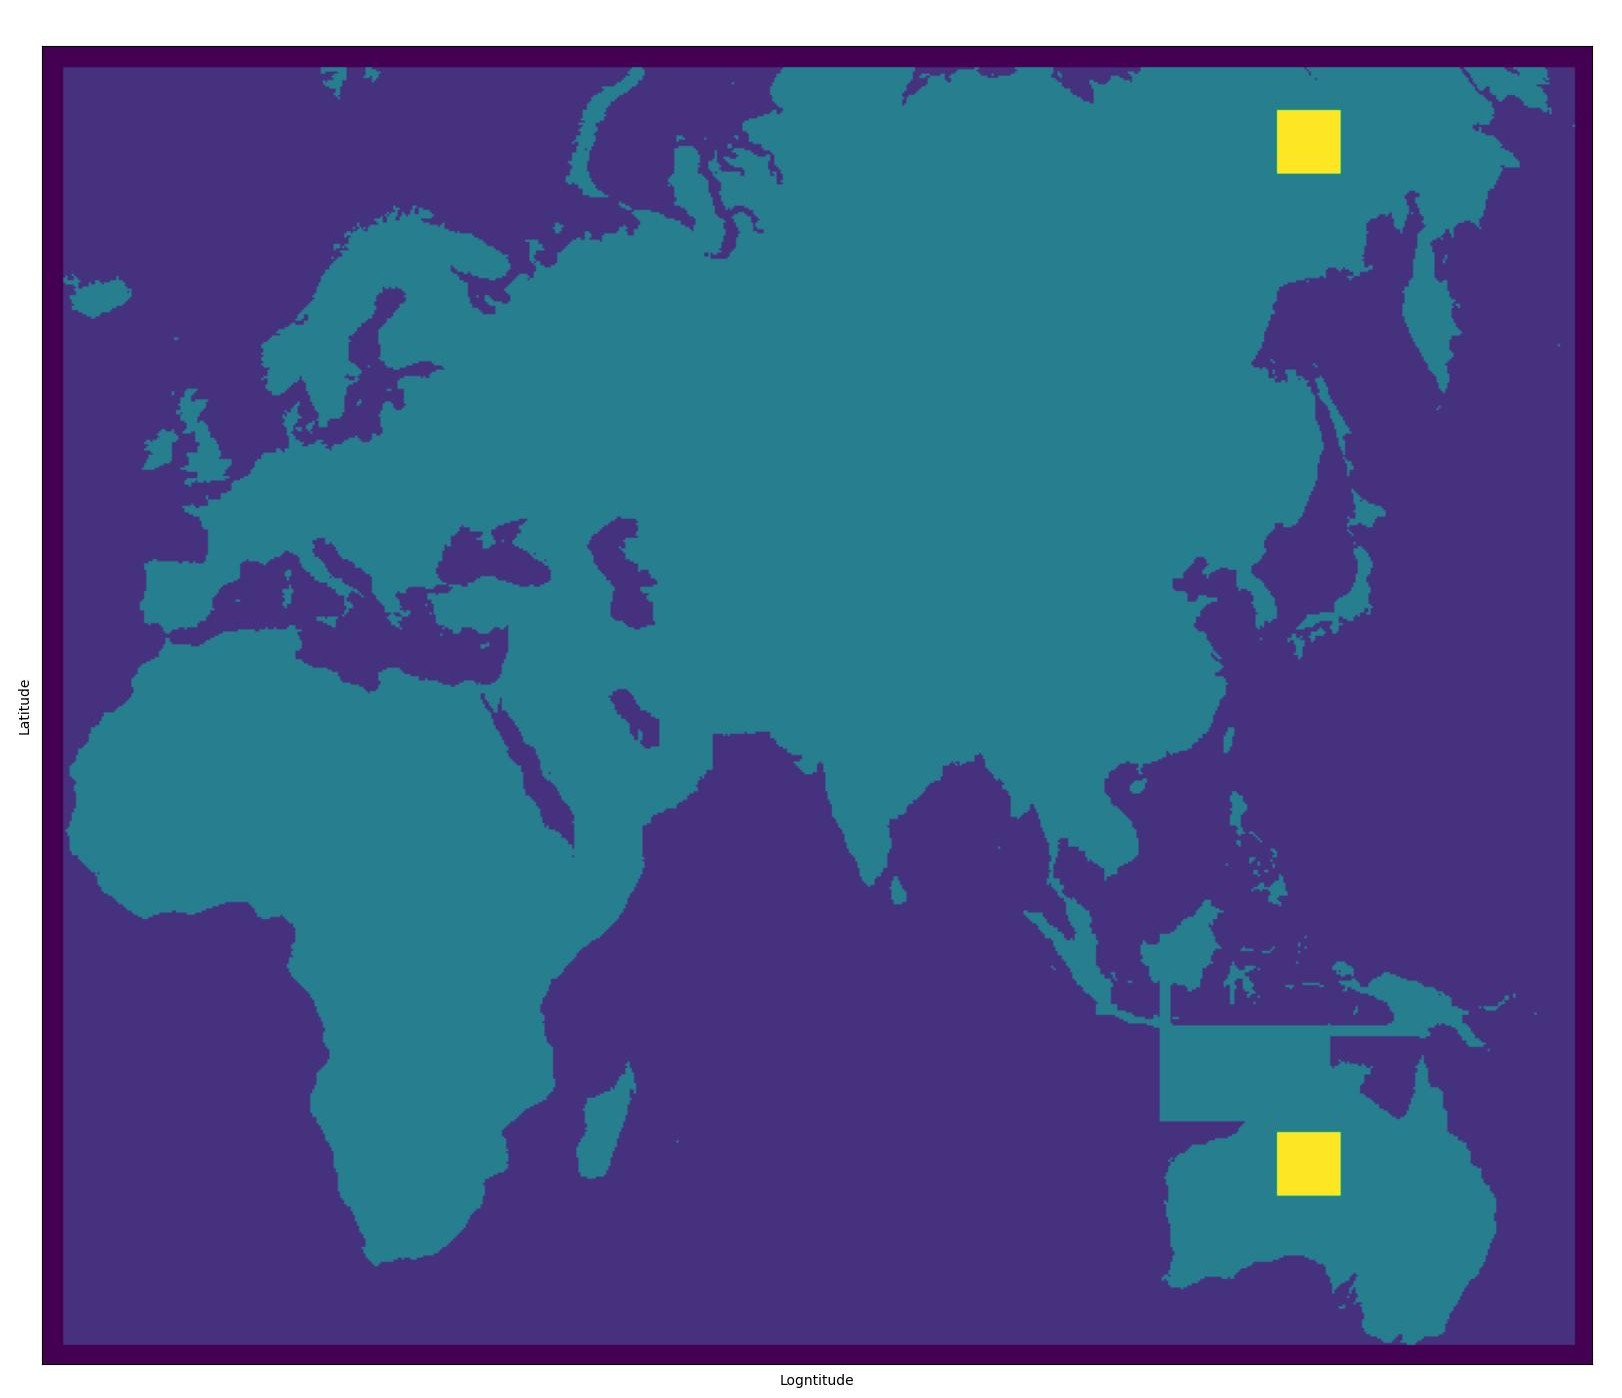
\includegraphics[scale=0.15]{Files/Images/reward_map.jpg}
        \caption{Reward map.}
    \end{minipage}
    
    \begin{minipage}{0.49\textwidth}
        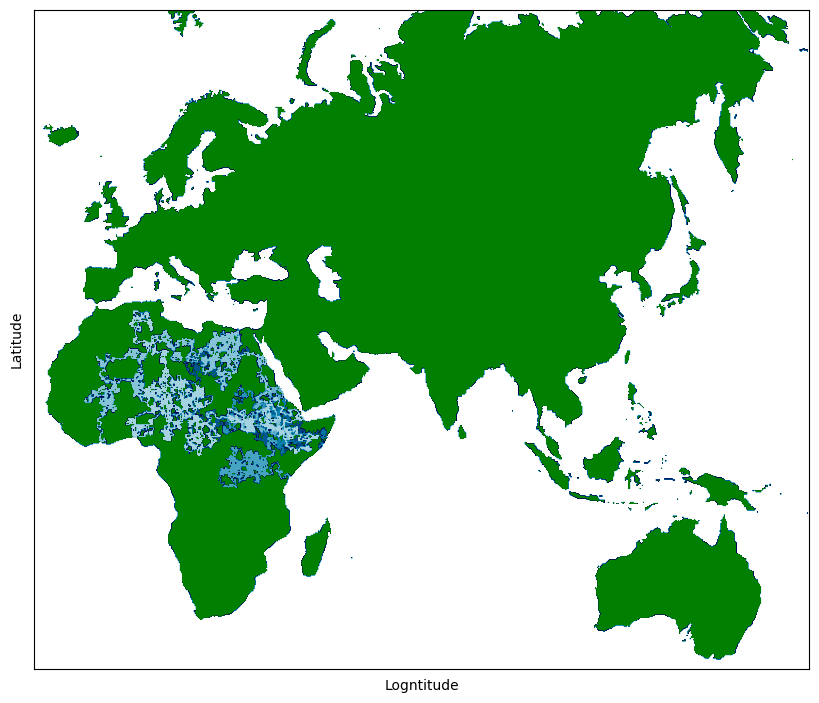
\includegraphics[scale=0.3]{Files/Images/random.png}
        \caption{Random walk of the agent in the early stages}
    \end{minipage}
    \begin{minipage}{0.49\textwidth}
        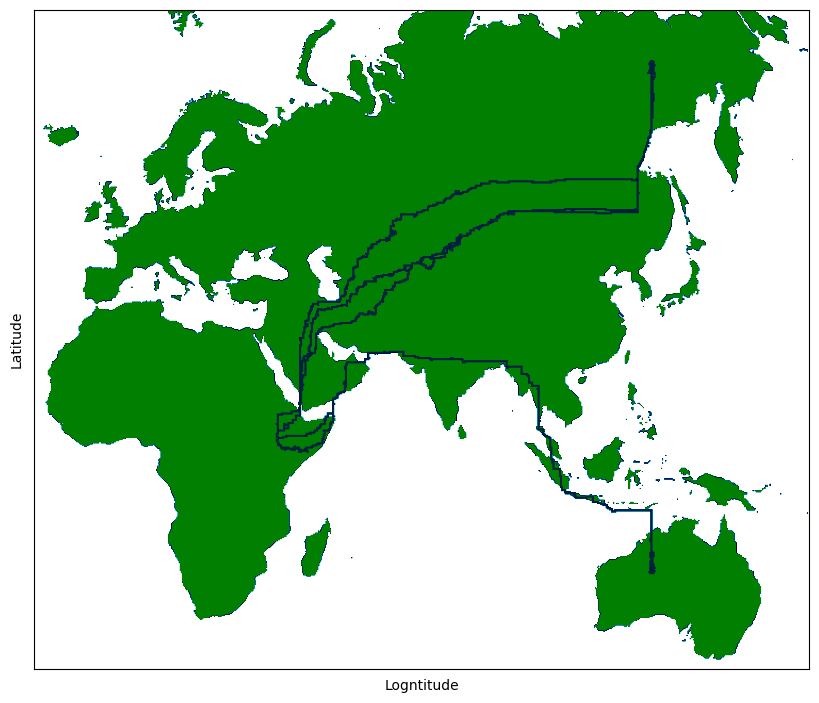
\includegraphics[scale=0.3]{Files/Images/optimised.png}
        \caption{Fully optimised agent.}
    \end{minipage}
    
    \begin{minipage}{0.49\textwidth}
        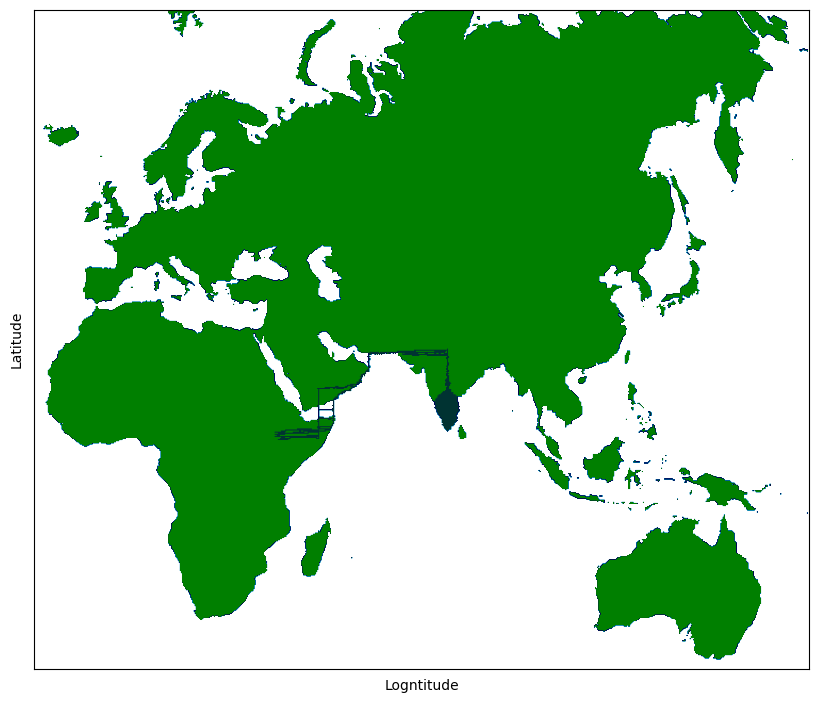
\includegraphics[scale=0.3]{Files/Images/greed.png}
        \caption{Showcase of the greediness of the Qlearning algorithm}
    \end{minipage}
    \begin{minipage}{0.49\textwidth}
        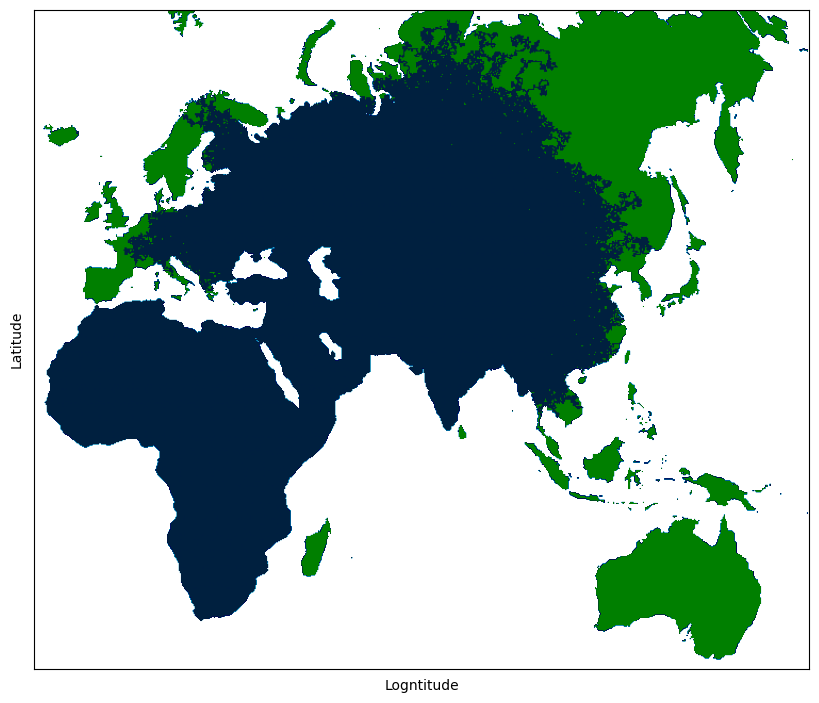
\includegraphics[scale=0.3]{Files/Images/inefficient.png}
        \caption{The agent hasn't found any reward point after $N=10000$ episodes.}
    \end{minipage}
\end{figure}

\begin{multicols}{2}
\subsection{Solutions to the Problem.}
There are multiple possible solutions to the problem of "unnaturalness" and greed. The first one is to implement a different method, such a genetic algorithm like ant colony optimization methods, whilst a second one could be to manually set negative reward areas in natural landmarks, like the Sahara Desert, the Caucasus, the Himalayas etc. This is cumbersome\footnote{Interestingly, this was the initial goal of this project. Based on the patterns of human migration, is an AI able to generate the real world environment in which they happened? Is it possible to generate for example the Sahara, by pointing out that humans stuck to the coastlines of Africa or went through the sea? Alas, the concept proved too challenging for this project and was thus scraped.}, not only due to the large number of natural environments that could be considered "natural obstacles", but also because the whole process approximately took 160 thousand years, meaning that the climate and landscape was constantly changing. An example of this is the Ice Ages, the changing ocean levels, the land bridge that allowed the first Humans to cross for Siberia into North America etc.\\
For this reason, we will implement the third option, which is to stop the training early, and lightly incentivize the agent to go to the wanted points through some clever manipulation of the whole process.\\

\subsubsection{Proposed Solution}
We introduce an "expendable" reward area, where once the agent reaches it, it changes it's reward value. This works so that the agent its never finding the same coordinates rewarding, incentivizing exploring. We also make it so once both those areas are empty of rewards we refill them so as to not have an empty reward map.\\
By letting the algorithm explore and discover Australia and the Bering Strait, and then allowing the agent to nearly optimise (this happens around the $N=210000$ episode, so we start the following plan at around $N=195000$), we create small reward points at the tip of India, as well as at Brunei and Papua New Guinea, since this make the whole process look more natural, due to the fact that they had to reach Australia by boats, and assuming they didn't have the naval technology or the maps to know where they were going, some groups might have ended up in those islands\footnote{In the final figure none of those seem to have been prefered but the still played a role in influencing the agent to train slower by "confusing" the agent.}. By also stopping the training before the optimisation point (we stop the training at $N=200000$ episodes) we get the final result (Fig. 8).
\end{multicols}
\begin{figure}[h!]
    \centering
    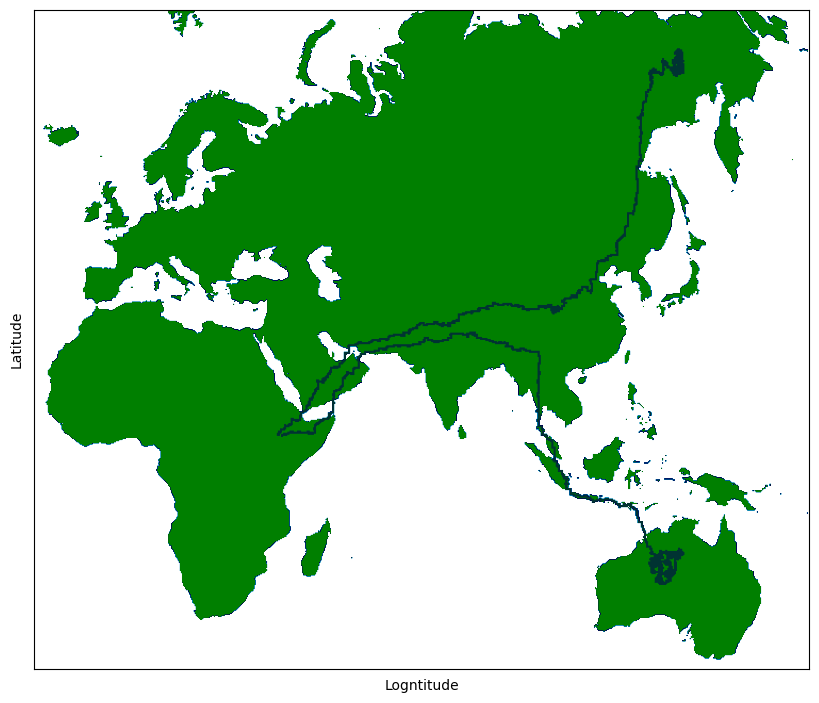
\includegraphics[scale=0.4]{Files/Images/final.png}
    \caption{A more probable and almost natural-looking paths to Australia and East Siberia}
    \label{fig:my_label}
\end{figure}

\begin{multicols}{2}
\subsection{Possible Improvements}
In theory the project could be further improved with some minor landscaping, adding the major landmarks, like the Sahara Desert and the Himalayas for example, as well as by making a more thorough search of the information on the subject, both in terms of dispersals of people, as well as geological and climatic data. To add these, we could manually add them and add a diffusion process to the entire map so that rewards have fuzzy borders around them, since this adds more realistic "natural boundaries" between the different biomes.\\
A dynamic reward map would not work since the agent has no prior idea to the map and so any changes it does not observe are meaningless in the matter of training the agent, although it would be more realistic, since humans didn't know or care about the climate of regions until they settled them.\\
The project also doesn't simulate the changing population of the groups, but rather is a single agent. Attempts were made to include a mechanism that after a fixed point of actions (say 50 years) would replace the agent  implying the death of the previous generation, and the continuation of the journey by the new one, but due to the nature of Qlearning, this yielded no improvements, and only added complexity to the code, so it was scrapped. It did however lay the idea of a genetic algorithm improving the simulation.
\section*{Acknowledgments}
In general this project has alot of room to improve on, both in theory and in execution, but unfortunately the constraints of this course limit me to 6 pages, which are just enough to display the work that I have done and also include the references, especially the work of Lopez, Van Drop, and Hellenthal\cite{EOBO} who's paper let me find the rest of the bibliography.
\newcolumn
\nocite{*}
\printbibliography
\end{multicols}

\end{document}